\subsection{Topologia del Sistema}

La topologia del sistema è rappresentata nel seguente schema:

\begin{figure}[h]
\centering
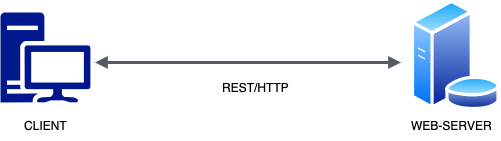
\includegraphics[scale=0.75]{images/topologia.png}
\caption{Diagramma dell’architettura della webapp Spendly}
\end{figure}

Il sistema è basato unicamente su un’architettura \textbf{web}, in cui i client interagiscono con un \textbf{web server} sviluppato in \textbf{Spring Boot}. I client utilizzano un browser, comunicando con il server attraverso \textbf{REST-API HTTP}, con dati in formato \textbf{JSON}. 

\subsubsection{Protocollo HTTP e REST-API}

HTTP è un protocollo di trasferimento ipertestuale che offre un meccanismo semplice e universale per inviare e ricevere dati. È ideale per le nostre REST-API poiché assicura la compatibilità con i browser e l’interscambio di dati in JSON su qualsiasi piattaforma.

\subsubsection{Caratteristiche dell’architettura}

\begin{itemize}
\item \textbf{Scalabilità}: possibilità di scalare l’intero sistema o le singole funzionalità in base alle necessità.
\item \textbf{Modularità}: sviluppo e manutenzione semplificati grazie all’organizzazione delle funzionalità in moduli indipendenti.
\item \textbf{Affidabilità}: eventuali malfunzionamenti in una funzionalità non compromettono l’intero sistema.
\item \textbf{Manutenibilità}: possibilità di aggiornare o sostituire singoli moduli senza interrompere l’operatività complessiva.
\end{itemize}